\chapter{Datastructure Octree}
\label{mise_en_oeuvre}

\paragraph{}
Pour la gestion des collisions et l'attraction/répulsion, la recherche du plus
proche voisin est utilisée pour chaque atome et pour chaque frame. Avec la
datastructure utilisée pour stocker les atomes (une ArrayList), pour chaque
atome on a alors une complexité en pire scénario de $O(N)$. Au total, pour tous
les atomes, on a alors une complexité en $O(N^2)$ pour chaque frame.

\paragraph{}
Dans l'ancienne implémentation séquentielle, la liste des atomes était
parcourue pour chaque frame de façon à mettre à jour les positions des atomes.
Utiliser une datastructure pour optimiser la recherche de voisins augmenterait
dans tous les cas la complexité du parcours des atomes. Le passage sur des
atomes Agents a changé la donne, puisqu'ils se mettent à jour eux même et
évitent le parcours de liste. Il y a alors tout intérêt à opter pour une
datastructure plus optimisée pour la recherche que pour le parcours.


\section{Choix de datastructure}

\paragraph{}
La nouvelle datastructure pour stocker les atomes se doit d'être optimisée pour
la recherche de voisins dans un environnement 3D. Les deux datastructures qui
ressortent sont l'Octree et le K-D Tree.

\subsection{Octree}

\paragraph{}
Un Octree est la version tridimensionnelle du Quadtree, reposant sur la
sous-division de cubes en 8 cubes enfants. Un cube contient un nombre
d'éléments maximum M. Dès que ce nombre est dépassé, le cube se subdivise en 8
cubes.

\begin{figure}[H]
\centering
\centerline{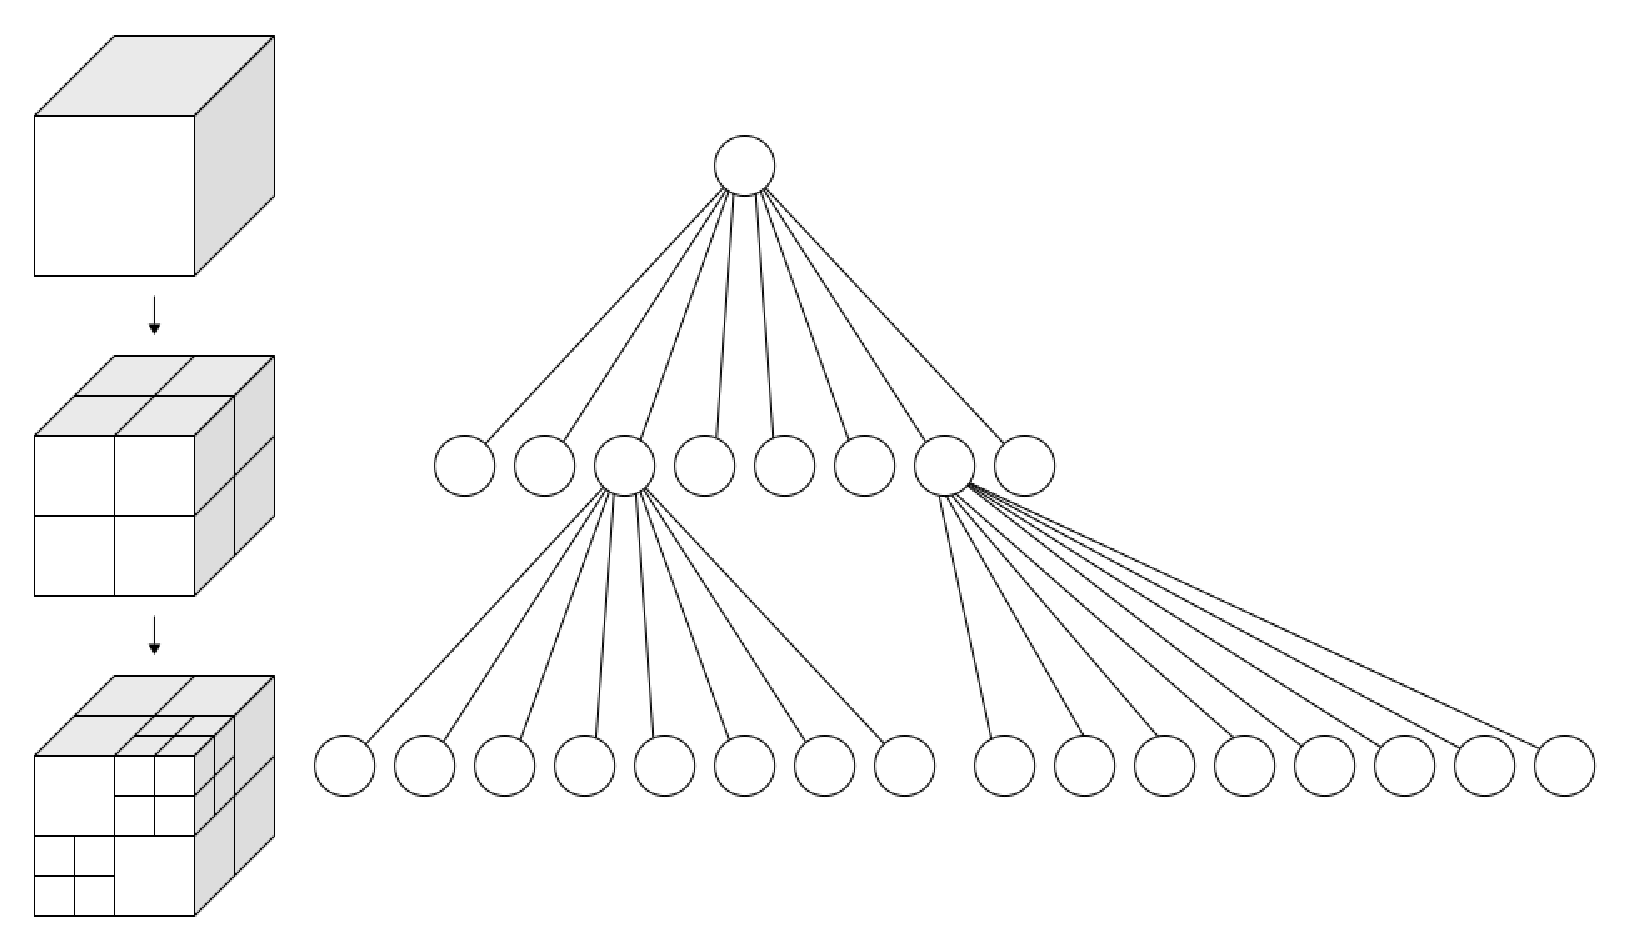
\includegraphics[width=0.8\textwidth]{octree.eps}}
\caption{Schéma de décomposition d'un octree}
\label{octree_img}
\end{figure}

\paragraph{}
Après sous-division, les objets sont éparpillés dans les cubes enfants en
fonction de leur position dans l'espace. Il s'agit, pour simplifier, de classer
les objets via une sorte de dichotomie pour chaque dimension, d'où les 8 cubes.
La recherche d'un élément via ses coordonnées est alors très rapide, puisque
les éléments sont disposés dans chaque cube en fonction de cette variable.


\subsubsection{Recherche de voisins}
\paragraph{}
Dans chaque cube, les éléments sont stockés dans une ArrayList de taille
maximum $M$, fixée et comprise entre 1 et $N$ ($N$ le nombre total d'éléments
stockés dans l'ensemble de l'octree). La recherche de voisins s'effectue en
cherchant les cubes entourant un objet. La recherche du plus proche voisin a
alors comme complexité dans le pire cas $O(27(M + N))$, soit environ $O(M+N)$.
$O(M)$ est ici la complexité à parcourir tous les éléments de chaque cube
(puisque cela revient à parcourir une ArrayList de taille $M$). $O(N)$
correspond à la complexité à atteindre un cube donné dans l'octree dans le pire
des cas. Ces deux complexités sont à multiplier par 27, qui correspond au
nombre maximum de cubes pouvant entourer un objet. Dans le cas où $M$ est fixée
à la même valeur que $N$, la complexité est de $O(2N)$ par atome, soit $O(N^2)$
pour avoir le plus proche voisin pour l'ensemble des $N$ atomes.

\paragraph{}
Le cas moyen est intéressant à étudier car montre le rôle que joue M dans
l'efficacité de l'algorithme. La complexité est de $O(M +
\frac{\log(N)}{3\log(M)\times{}\log(2)})$, soit environ $O(M +
\frac{\log(N)}{\log(M)})$. On négligera le nombre de cubes entourant l'élément
puisqu'il n'impacte que peu la complexité finale. $O(M)$ est ici encore la
complexité à parcourir tous les éléments d'un cube (ArrayList de taille $M$).
$O(\frac{\log(N)}{\log(M)})$ correspond ici à la complexité d'accéder à un cube
donné. Le nombre de cubes moyen entourant un objet est ici négligé. Si $M$ se
rapproche de 1, la complexité est environ de $O(N)$ par atome, soit $O(N^2)$
pour l'ensemble des atomes. La complexité est environ la même si $M = N$.
Néanmoins, il est plus avantageux que $M$ soit égal à $N$ plutôt qu'à 1, à
cause du nombre de cubes entourant l'objet pas mis en évidence ici car non pris
en compte dans les calculs.

\paragraph{}
On s'aperçoit alors que l'Octree est avantageux pour la recherche de voisins,
mais il est important de fixer une valeur appropriée pour le nombre maximum
d'éléments par cube, auquel cas la complexité sera plus mauvaise que celle
d'une ArrayList. Fixer un $M$ trop faible reviendra à obtenir énormément de
cubes, puisqu'un cube ne pourra contenir que peu d'éléments, ce qui rendra lent
l'accès à un cube donné. Fixer un $M$ trop proche de $N$ rendra l'octree
inefficace, car sera composé de très peu de cubes contenant un grand nombre
d'éléments.


\subsubsection{Déplacement d'éléments}
\paragraph{}
Les nœuds de l'arbre dépendent des coordonnées des points, donc déplacer un
point peut amener à déplacer un nœud. Contrairement à l'arbre k-d, cette étape
n'est pas forcément nécessaire, et le déplacement léger d'un atome ne
requièrera pas, dans la plupart des cas, d'être déplacé dans un autre cube.  On
aura alors dans la plupart des cas une complexité de $O(1)$ pour le déplacement
d'un atome, et au pire $O(N)$ ($O(2N)$ pour accéder au cube de l'élément à
déplacer puis le supprimer de l'ArrayList, $O(2N)$ pour l'insérer dans le cube
approprié à ses nouvelles coordonnées). Également, un octree n'a pas besoin
d'être équilibré. Ces deux points en font un arbre intéressant pour le cas de
la simulation d'atomes, où les éléments sont sans cesse en mouvement.


\subsubsection{Choisi comme datastructure principale}
\paragraph{}
L'octree a été choisi comme datastructure servant à stocker ses atomes pour sa
facilité d'implémentation comparé à un arbre k-d, la rapidité en moyenne à
déplacer un élément et la complexité de la recherche de voisin le plus proche,
qui permet d'être au pire quasiment aussi efficace qu'une ArrayList, et dans le
meilleur des cas permet de se rapproche d'une complexité en $O(\log(N))$ par
élément, soit $O(N\log(N))$ pour l'ensemble des atomes, lorsque la variable $M$
est correctement fixée et $N$ assez grand.

\subsection{K-D Tree}

\paragraph{}
Un K-D tree est un arbre binaire, équilibré. La complexité en cas moyen pour de
la recherche de voisins est de $O(log(N))$, pire cas $O(N)$. Comme pour
l'octree, les nœuds de l'arbre dépendent des coordonnées des points, donc ici
déplacer un point revient à déplacer un nœud et à re-balancer l'arbre. Ce point
est important car nous sommes ici dans un environnement où les atomes sont
constamment en mouvement.  La complexité d'insertion d'élément est en moyenne
de $O(log(N))$, ce qui est également le cas pour la suppression. Bouger un
élément dans l'arbre a alors une complexité de $O(2log(N))$.

\paragraph{}
Pour chaque frame, en cas moyen, la méthode de recherche de voisin ainsi que le
déplacement d'atome aurait une complexité de $O(3log(N))$, et comme pire cas
$O(3N)$. Au total, pour tous les atomes, la complexité totale serait alors de
$O(Nlog(N))$ en cas moyen et $O(N^2)$ en pire cas. Cela reste inférieur à la
complexité de l'ArrayList en cas moyen, mais il faut atteindre un grand nombre
d'atomes pour que la différence soit intéressante, c'est pourquoi la solution
n'a pas été retenue.


\section{Implémentation}

\subsection{StampedLock}
\paragraph{}
Avec des atomes agents, il est nécessaire que l'octree soit threadsafe tout en
étant performant pour plusieurs centaines voir milliers d'accès ou écritures
simultanées. L'approche choisie a donc été d'utiliser un système de lock
permettant de passer un cube en read-only ou de le bloquer complètement lors
de l'ajout ou suppression d'éléments. Il est également important de profiter du
système d'arbre, où les locks peuvent être localisés : il est possible de lock
uniquement une branche de l'arbre et les cubes qui la composent sans avoir à
lock tout l'octree.

\paragraph{}
Les StampedLock ont paru être la meilleure solution, car ils amènent un couple
de lock read/write : le ReadLock est ré-entrant, même entre threads, par contre
le WriteLock ne l'est pas. Cela permet des accès simultanés en lecture dans
l'octree, tout en bloquant les demandes d'écriture le temps que l'accès soit
terminé, mais aussi l'inverse en évitant les écritures simultanées, et en
bloquant les demandes de lecture le temps que les modifications soient
terminées. De plus, les StampedLock ont de meilleures performances que les
ReadWriteReentrantLock.


\begin{figure}[H]
\begin{lstlisting}
public ArrayList<T> getObjects() throws InterruptedException {
    if(isLeaf())
        return new ArrayList<T>(objects);

    ArrayList<T> childrenObjects = new ArrayList<T>();
    long stamp = 0;
    try {
        stamp = rwlock.readLockInterruptibly();
    } catch (InterruptedException e) {
        e.printStackTrace();
        return childrenObjects;
    }

    try {
        for (Octree<T> child : children) {
            if (child.hasObjects())
                childrenObjects.addAll(child.getObjects());
        }
    } finally {
        rwlock.unlockRead(stamp);
    }

    return childrenObjects;
}
\end{lstlisting}
\caption{Exemple d'utilisation de read lock}
\label{octree_code_getobjects}
\end{figure}

\paragraph{}
Ce bloc prend comme exemple le retour des objets d'un cube, qui le place en
read-only le temps de rassembler tous les objets des enfants, évitant toute
écriture.

\paragraph{}
Des tests unitaires permettent de tester la caractéristique thread-safe de
l'octree, en créeant plusieurs threads qui effectuent des modifications
simultanées dans l'arbre. L'intérêt est de simuler le comportement qu'auront
les atomes avec l'arbre pendant l'exécution du programme.


\subsection{Recherche du plus proche voisin}

\paragraph{}
Pour la recherche de voisins, deux méthodes ont été implémentées : recherche de
tous les atomes dans une certaine zone (que l'on appellera recherche via
sphère), ou en recherchant dans tous les cubes entourant le cube dans lequel se
trouve l'élément.

\subsubsection{Recherche via une sphère}
\paragraph{}
La méthode de la sphère pour chercher le voisin le plus proche d'un élément
consiste à choisir un second élément au hasard contenu dans le même cube. Ceci
dû, elle fonctionne uniquement si le cube contient plus d'un élément, dans le
cas contraire on basculera sur la méthode de recherche des cubes aux alentours.
L'objectif est d'obtenir tous les éléments contenus dans la sphère dont le
centre est notre élément, et ayant comme rayon la distance entre le premier
et le second élément.

\paragraph{}
Si la sphère sort du cube actuel, un calcul est fait pour déterminer quels
cubes voisins font partie de la sphère. Dans tous les voisins retournés, la
distance pour chaque est calculée avec le centre de la sphère (l'élément pour
lequel on souhaite trouver le plus proche voisin), et celui ou ceux pour qui la
distance est la plus faible sont gardés et considérés comme plus proche
voisins.

\paragraph{}
L'intérêt par rapport à la méthode suivante est que le nombre de voisins à
évaluer est en théorie bien inférieur. Le nombre de distance à calculer est
alors réduit.

\subsubsection{Recherche via les cubes voisins}
\paragraph{}
La méthode via les cubes voisins consiste sur la détermination des cubes étant
en contact avec le cube de l'élément visé. Pour se faire, l'algorithme va
trouver chaque cube ayant une arrête partagée avec le cube actuel, ce qui donne
au maximum 27 cubes voisins. Très peu de calculs sont nécessaires, ils sont
trouvés très rapidement. L'accès aux cubes voisins est cependant plus long, ce
qui donne la complexité donnée dans la partie détaillant le choix de l'octree.

\paragraph{}
Une fois les cubes voisins obtenus, pour chaque objet les constituants ainsi
que ceux du cube actuel, la distance est évaluée avec l'élément ciblé, et le ou
les objets ayant la distance la plus faible sont gardés et considérés comme
plus proches voisins.

\paragraph{}
L'inconvénient de cette méthode par rapport à la recherche via une sphère est
que d'avantage de distances sont à calculés, puisqu'aucun filtre n'est effectué
en amont. Cela peut être un soucis si le nombre d'éléments maximum par cube est
élevé.

\subsubsection{Comparaison des performances}
\paragraph{}
De façon à s'assurer que les performances des algorithmes soient
satisfaisantes, des tests unitaires ont été écrits pour comparer le temps de
d'exécution d'algorithmes naïfs comparés aux différents algorithmes présentés.

\paragraph{}
\begin{figure}[H]
\begin{lstlisting}
@Test
public void getFarthestNeighbours() throws Exception {
    Environment environment = genEnvironment(1000, false);
    ArrayList<Atom> atoms = environment.getAtoms().getObjects();
    for(Atom a : atoms)
        octree.add(a);

    Atom atom = atoms.get(0);

    double start_naive_algorithm_time = stopwatch.runtime(TimeUnit.MICROSECONDS);
    ArrayList<Atom> farthestNeighsWithNaiveAlgorithm = new ArrayList<>();
    farthestNeighsWithNaiveAlgorithm.add(atoms.get(1));
    double farthestDistanceWithNaiveAlgorithm = atom.distance(atoms.get(1));
    for(Atom a : atoms) {
        double distanceAtomA = atom.distance(a);
        if(a != atom && distanceAtomA < farthestDistanceWithNaiveAlgorithm) {
            farthestDistanceWithNaiveAlgorithm = distanceAtomA;
            farthestNeighsWithNaiveAlgorithm = new ArrayList<>();
            farthestNeighsWithNaiveAlgorithm.add(a);
        }
        else if(distanceAtomA == farthestDistanceWithNaiveAlgorithm)
            farthestNeighsWithNaiveAlgorithm.add(a);
    }
    double naive_algorithm_time = stopwatch.runtime(TimeUnit.MICROSECONDS) - start_naive_algorithm_time;

    double start_algorithm_time = stopwatch.runtime(TimeUnit.MICROSECONDS);
    ArrayList<OctreePoint> farthestNeigh = octreeDistanceHelper.getFarthestNeighbours(octree, atom);
    double algorithm_time = stopwatch.runtime(TimeUnit.MICROSECONDS) - start_algorithm_time;
\end{lstlisting}
\end{figure}
\begin{figure}[H]
\begin{lstlisting}
    assertTrue(naive_algorithm_time >= algorithm_time);
    assertEquals(
        farthestDistanceWithNaiveAlgorithm,
        ((Atom) farthestNeigh.get(0)).distance(atom),
        0.001
    );
}
\end{lstlisting}
\caption{Test unitaire sur la recherche du plus proche voisin via les cubes
    environnants}
\label{octree_getFarthestNeighbours}
\end{figure}

\paragraph{}
Pour la recherche de voisins, l'algorithme naïf correspond à parcourir une
liste d'atomes et de garder les éléments pour lesquels la distance calculée est
la plus faible. Ici, le temps d'exécution est comparé avec la méthode de
recherche via les cubes voisins. Ici, sur notre machine de test, l'algorithme
naïf prend 2.8ms, quand l'algorithme par les cubes voisins prend 2ms pour un
environnement de 1000 éléments.

\paragraph{}
Grâce à ces tests, il a été mis en évidence que la recherche du plus proche
voisin est plus efficace via la méthode des cubes voisins que via la méthode de
la sphère. Cette dernière était, au mieux, 2 fois plus lente que la méthode
naïve, quand la première est au pire 1.5 fois plus lente, mais la plupart des
cas sont plus rapides, et certains tests ont montré des résultats étant 10 fois
plus efficaces.

\paragraph{}
Le résultat est étonnant car l'on s'attend à ce que le filtre effectué par la
méthode via une sphère allait la rendre plus efficace car réduit grandement le
nombre de distances à calculer. Finalement, le calcul est fait efficacement en
java, et c'est pourquoi la méthode des cubes voisins a été retenue pour la
recherche de voisin le plus proche.
